\documentclass[a4paper]{article}

\usepackage[portuguese]{babel}
\usepackage[utf8]{inputenc}
\usepackage{indentfirst}
\usepackage{graphicx}
\usepackage{verbatim}
\usepackage[T1]{fontenc}

\begin{document}

\setlength{\textwidth}{16cm}
\setlength{\textheight}{22cm}

\title{\Huge\textbf{Jogos de tabuleiro}\linebreak\linebreak\linebreak
\Large\textbf{Relatório 2ª Fase}\linebreak\linebreak

\includegraphics[height=6cm, width=7cm]{feup.pdf}\linebreak \linebreak
\Large{Mestrado Integrado em Engenharia Informática e Computação} \linebreak \linebreak
\Large{Base de dados}\linebreak
}

\author{\textbf{Grupo 601:}\\ Hugo Ari Rodrigues Drumond --- 201102900 \\  Ricardo Jorge Matos Figueiredo --- 201100687 \\ Gustavo Assis Freitas --- 200602187\\\linebreak\linebreak \\
 \\ Faculdade de Engenharia da Universidade do Porto \\ Rua Roberto Frias, 4200--65 Porto, Portugal \linebreak\linebreak\linebreak
\linebreak\linebreak\vspace{1cm}}
\maketitle
\thispagestyle{empty}

\newpage

%Decidimos elaborar uma base de dados para uma Empresa organizadora de \textit{Jogos de tabuleiro}.    \cite{creator}


%Descrever muito sumariamente (1-2 parágrafos) o trabalho que está a ser reportado

%\section{Introdução}

%Descrever os objectivos e motivação do trabalho.
%Todas as figuras devem ser referidas no texto. %\ref{fig:codigoFigura}

\section{Contexto}
Esta base de dados destina-se a um Salão de jogos que organiza jogos de Tabuleiro e foi desenvolvida, inicialmente, pensando num só jogo, o xadrez. Posteriormente, então, foi feita uma generalização. Em suma, são guardados os dados dos jogadores e dos torneios de uma dada temporada. Isto, possibilitará aos utilizadores da base de dados: rigor ao planear eventos, versatilidade, facilidade de registo, entre outros. Por exemplo, se eu quisesse organizar um torneio, em condições, iria ter saber à priori: os escalões, o jogo a que diz respeito, a temporada, as equipas inscritas e os patrocinadores. E registá-los em algum sítio para que depois possa associá-los, direta ou indiretamente, a uma partida e uma partida a equipas. A nossa base de dados tem como único propósito tornar esse \{pré,pós\}registo trivial.

%explicar de forma legível o nosso diagrama de classes uml melhorado. Tal como é feito nos primeiros exercícios.
\section{Conceitos Principais}
Num torneio de jogos de tabuleiro podem haver várias partidas entre duas ou mais equipas num dado escalão de um torneio. As partidas podem ocorrer em diversos sítios, têm de ser reguladas por um ou mais árbitros qualificados para o jogo em disputa e os resultados devem ser guardados. Cada equipa é formada por um ou mais jogadores. Podem haver vários torneios exatamente iguais, independentemente de quaisquer condicionantes.

%explicar como fizemos o mapeamento para o modelo relacional e qual o nível de normalização.
\section{Passagem ao modelo relacional e normalização}
A transição do diagrama de classes para o schema da base de dados foi feita sem grandes problemas. Optámos por separar a generalização em duas tabelas segundo o estilo orientado a objetos, porque ao fazer isto ficamos no ponto de equilibro entre poupar nas ligações de tabelas e nos recursos de armazenamento. Uma relação, menos ligações embora haja desperdício de armazenamento; Três relações, mais ligações e mesmo uso de recursos de armazenamento. A única ternária no nosso uml foi decomposta em EquipaPatrocinadorTorneio e a classe de associação em EquipaPartida. Mais as tabelas de "apoio". Na tabela Jogador o idPais->País tem o significado de Nacionalidade e idCidade->Cidade é um apontador para uma cidade que por sua vez está associada a um País. O telefone e a extensão podem não estar ligados nem ao País nem à morada de uma Pessoa, por isso não servem de determinante para nenhum desses atributos.
\\\newline
\textbf{Jogador}(\underline{idJogador}, nome, codigoPostal, dataNascimento, numeroAndar, rua, telefone, idPais->Pais, idCidade->Cidade, idExtensao->Extensao, email) \\
\textbf{Equipa}(\underline{nome}, abreviatura) \\ %dúvida aqui sobre bcnf
\textbf{JogadorEquipa}(\underline{idEquipa->Equipa}, \underline{idJogador->Jogador}) \\
\textbf{Árbitro}(\underline{idÁrbitro}, nome, codigoPostal, dataNascimento, numeroAndar, rua, telefone, idPais->Pais, idCidade->Cidade, idExtensao->Extensao, observacoes) \\
\textbf{LocalEncontro}(\underline{idLocalEncontro}, idCidade->Cidade, idExtensao->Extensao, codigoPostal, rua, telefone) \\
\textbf{Cidade}(\underline{idCidade}, nome, idPais->Pais) \textbf{TipoJogo}(\underline{nome}) \\
\textbf{ArbitroTipoJogo}(\underline{idArbitro->Arbitro}, \underline{idTipoJogo->TipoJogo}) \\
\textbf{Partida}(\underline{idPartida}, dataInicio, duracao, idEscalao->Escalao) \\
\textbf{ArbitroPartida}(\underline{idArbitro->Arbitro}, \underline{idPartida->Partida}) \\
\textbf{EquipaPartida}(\underline{idEquipa->Equipa}, \underline{idPartida->Partida}, posicao, resultado) \\
\textbf{Patrocinador}(\underline{nome}) \textbf{Escalao}(\underline{nome}) \\
\textbf{EquipaPatrocinadorTorneio}(\underline{idEquipa->Equipa}, \underline{idPatrocinador->Patrocinador}, \underline{idTorneio->Torneio}) \\
\textbf{Torneio}(\underline{idTorneio}, idTipoJogo->TipoJogo, nome, temporada, formato) \\
\\\newline
A nossa base de dados de início encontra-se na 3ª Forma Normal, visto que respeita a 1ª, 2ª, 3ª formas normais. Deste modo a nossa base de dados evita algumas anomalias: redundância de dados, atualização de campos, campos sinónimos, entre outros. Não continuámos a normalizar para além da 3ª Forma Normal porque isto tornaria a nossa base de dados mais lenta devido à quantidade de ligações, mais difícil de pesquisar e por não ser exigido pelos docentes. Todas as nossas relações estão na 1ª Forma Normal porque são respeitadas as regras das tabelas e porque em cada relação está definida uma chave primária. Também está na 2ª visto que nenhum subconjunto das chaves primárias determina um atributo não chave, as nossas relações só têm uma chave ou são todas chaves portanto respeitam de imediato esta Forma Normal. Excepto a classe de associação que é necessário identificar se um subconjunto da chave identifica um atributo não chave, que não se verifica, portanto está na segunda Forma Normal. Para respeitar a 3ª Forma Normal não podem haver dependências funcionais transitivas, A->B \&\& B->C, que não acontece na nossa bases de dados. A única razão para a nossa base de dados não respeitar a BCNF restringe-se às relações Árbitro e Jogador, porque existe um determinante em cada uma das relações que não é chave candidata, a dependência funcional idCidade->Cidade,rua -> codigoPostal. Cada Cidade tem um nome, um apontador para um País e um código único que serve de chave. Uma maneira de corrigir isto seria criar uma nova tabela chamada CidadeRua em que iria existir uma chave estrangeira, idCidade->Cidade, e um membro chamado rua. Estes dois campos funcionariam como chaves primárias nesta tabela e identificariam o codigoPostal. Nas outras duas tabelas haveria uma chave estrangeira chamada idCidadeRua->CidadeRua e seriam removidos os campos codigoPostal, idCidade->Cidade e rua.

%indicar o tipo de restrições que foram usadas e a criação das tabelas
\section{Linguagem de Definição de dados e Restrições}
Na nossa base de dados existem algumas restrições e gatilhos.
Restrições de valor: NOT NULL, limites de atributo.
Restrições de atributos: ainda não temos, temos de arranjar maneira de colocar isto em qualquer lado
Asserção: arranjar uma maneira de colocar isto
E obviamente que foram definidas chaves primárias e estrangeiras que são um tipo de restrição.

%Dizer o que irá ser inserido na bases de dados
\section{Linguagem de Manipulação de dados}

%Incluir todas as restrições, digitalizar o diagrama ou fazer num programa qualquer. Incluir notas.
\section{Diagrama de classes UML melhorado}
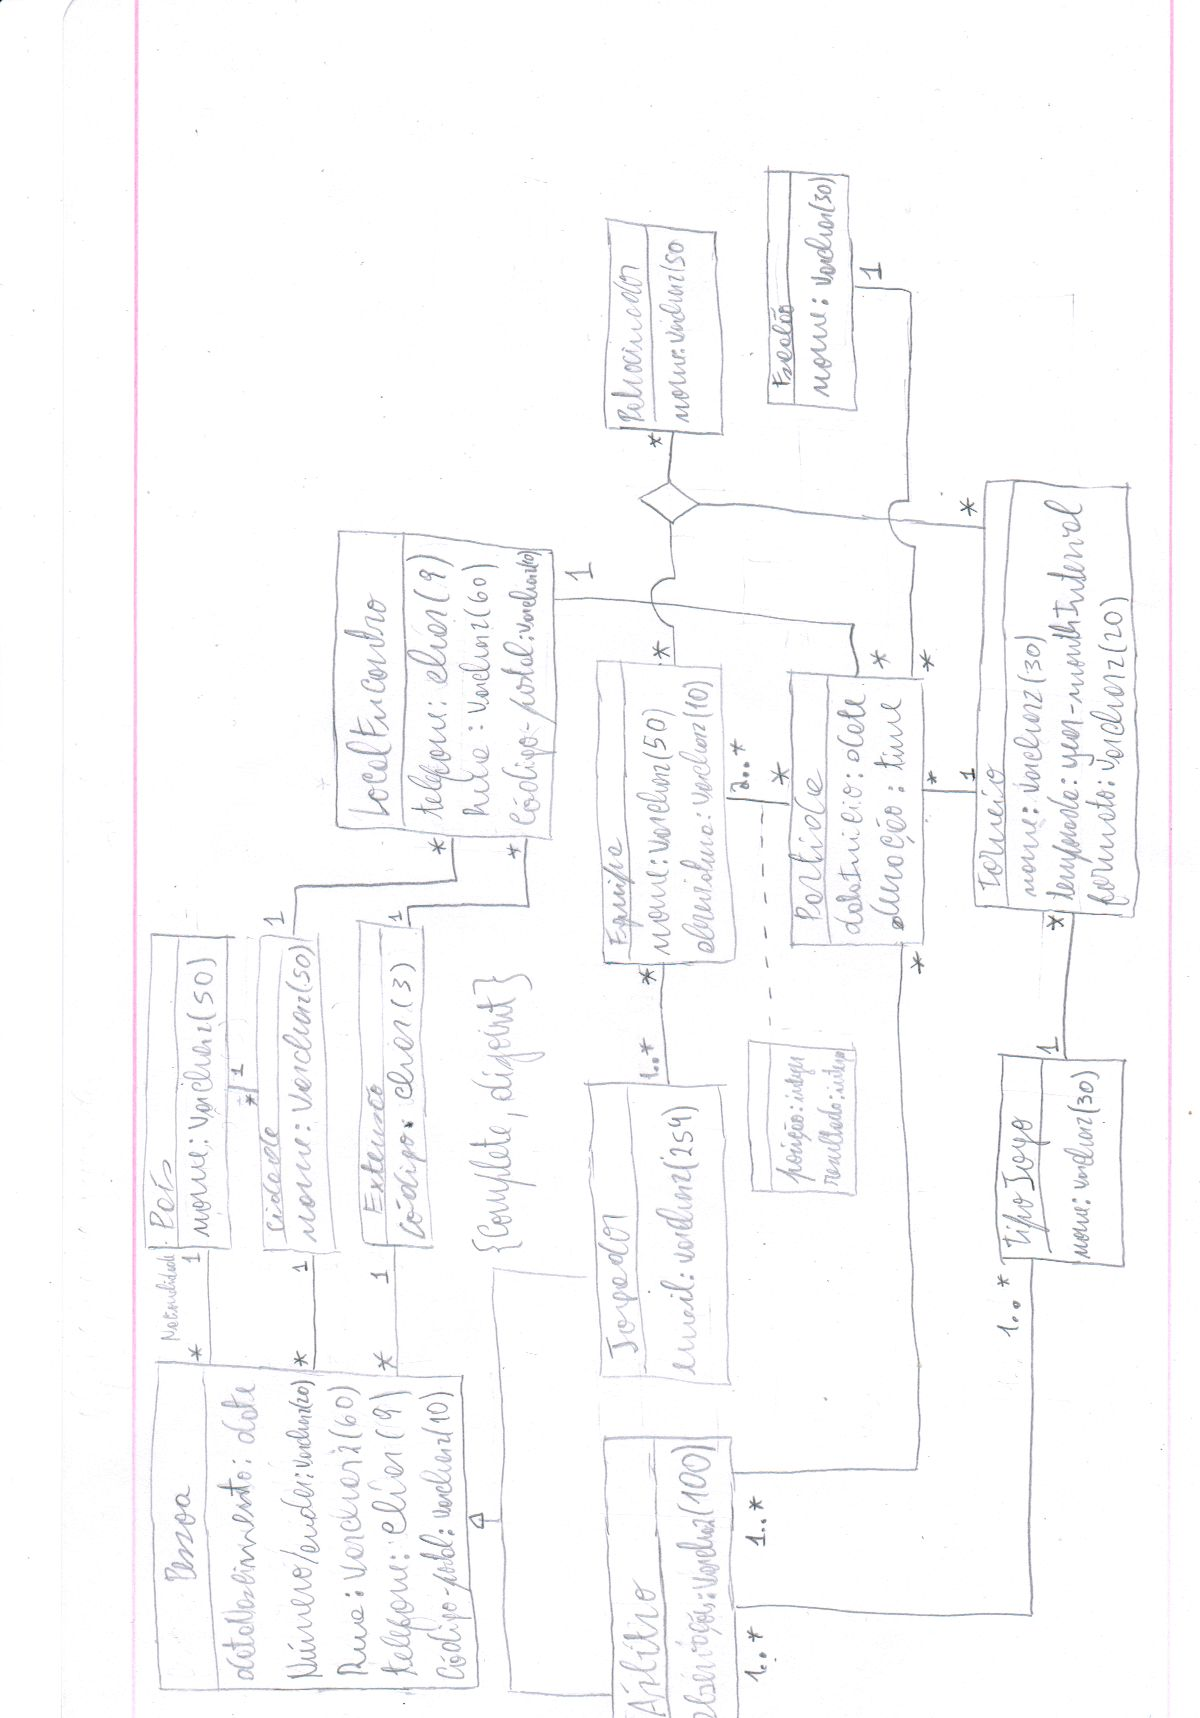
\includegraphics[scale=0.6]{./BDAD_DIAGRAMA_CORRIGIDO.jpeg}
\end{document}
